% !TeX document-id = {efee450f-6069-4a1d-a54f-d3ae0eb7270d}
% !TeX TXS-program:compile = txs:///pdflatex/[-shell-escape]

\documentclass[11pt]{beamer}
\usepackage[utf8]{inputenc}
\usepackage[T1,T2A]{fontenc}
\usepackage[russian]{babel}
\usepackage{color}
\usepackage{listings}
\usepackage{calc}
\usepackage{graphicx}
\usepackage{epstopdf}
\usepackage{hyperref}
\hypersetup{unicode,colorlinks}
\usepackage{csquotes}
\usepackage{upquote}
\usepackage{cprotect}
\usetheme[progressbar=head,numbering=fraction,block=fill]{metropolis}
\usepackage{dejavu}
\usepackage{etoolbox}
\usepackage{bm}
\usepackage{minted}
%\usepackage[defaultsans]{droidsans}
%\usepackage[defaultmono]{droidmono}
%\makeatletter
%\input droid/t1fdm.fd
%\makeatother

\makeatletter
\DeclareRobustCommand*{\bfseries}{%
    \not@math@alphabet\bfseries\mathbf
    \fontseries\bfdefault\selectfont
    \boldmath
}
\makeatother

\makeatletter
\chardef\straightquote@code=\catcode`'
\chardef\backquote@code=\catcode``
\catcode`'=\active \catcode``=\active
\patchcmd{\@noligs}
{\textasciigrave}
{\fixedtextasciigrave}
{}{}
\newcommand{\fixedtextasciigrave}{%
    \makebox[.5em]{\fontencoding{TS1}\fontfamily{fvs}\selectfont\textasciigrave}% Vera Sans
}
\catcode\lq\'=\straightquote@code
\catcode\lq\`=\backquote@code
\makeatletter

\lstset{
    language=Haskell,
    inputencoding=utf8,
    extendedchars=true,
    breaklines=true,
    escapeinside=!!,
    tabsize=4,
    breakatwhitespace=true,
    keepspaces=true,
    basicstyle=\ttfamily,
    commentstyle=\color{gray}\itshape,
    keywordstyle=
    % keywordstyle=\color{blue}, % TODO https://tex.stackexchange.com/questions/415777/avoid-highlighting-keywords-following-certain-words-in-listings
    % addkeywords={Type}
    % deletekeywords={Monad, String, return, array, show},
    % otherkeywords={::, ->}
}
\lstset{
    literate={а}{{\selectfont\char224}}1
    {б}{{\selectfont\char225}}1
    {в}{{\selectfont\char226}}1
    {г}{{\selectfont\char227}}1
    {д}{{\selectfont\char228}}1
    {е}{{\selectfont\char229}}1
    {ё}{{\"e}}1
    {ж}{{\selectfont\char230}}1
    {з}{{\selectfont\char231}}1
    {и}{{\selectfont\char232}}1
    {й}{{\selectfont\char233}}1
    {к}{{\selectfont\char234}}1
    {л}{{\selectfont\char235}}1
    {м}{{\selectfont\char236}}1
    {н}{{\selectfont\char237}}1
    {о}{{\selectfont\char238}}1
    {п}{{\selectfont\char239}}1
    {р}{{\selectfont\char240}}1
    {с}{{\selectfont\char241}}1
    {т}{{\selectfont\char242}}1
    {у}{{\selectfont\char243}}1
    {ф}{{\selectfont\char244}}1
    {х}{{\selectfont\char245}}1
    {ц}{{\selectfont\char246}}1
    {ч}{{\selectfont\char247}}1
    {ш}{{\selectfont\char248}}1
    {щ}{{\selectfont\char249}}1
    {ъ}{{\selectfont\char250}}1
    {ы}{{\selectfont\char251}}1
    {ь}{{\selectfont\char252}}1
    {э}{{\selectfont\char253}}1
    {ю}{{\selectfont\char254}}1
    {я}{{\selectfont\char255}}1
    {А}{{\selectfont\char192}}1
    {Б}{{\selectfont\char193}}1
    {В}{{\selectfont\char194}}1
    {Г}{{\selectfont\char195}}1
    {Д}{{\selectfont\char196}}1
    {Е}{{\selectfont\char197}}1
    {Ё}{{\"E}}1
    {Ж}{{\selectfont\char198}}1
    {З}{{\selectfont\char199}}1
    {И}{{\selectfont\char200}}1
    {Й}{{\selectfont\char201}}1
    {К}{{\selectfont\char202}}1
    {Л}{{\selectfont\char203}}1
    {М}{{\selectfont\char204}}1
    {Н}{{\selectfont\char205}}1
    {О}{{\selectfont\char206}}1
    {П}{{\selectfont\char207}}1
    {Р}{{\selectfont\char208}}1
    {С}{{\selectfont\char209}}1
    {Т}{{\selectfont\char210}}1
    {У}{{\selectfont\char211}}1
    {Ф}{{\selectfont\char212}}1
    {Х}{{\selectfont\char213}}1
    {Ц}{{\selectfont\char214}}1
    {Ч}{{\selectfont\char215}}1
    {Ш}{{\selectfont\char216}}1
    {Щ}{{\selectfont\char217}}1
    {Ъ}{{\selectfont\char218}}1
    {Ы}{{\selectfont\char219}}1
    {Ь}{{\selectfont\char220}}1
    {Э}{{\selectfont\char221}}1
    {Ю}{{\selectfont\char222}}1
    {Я}{{\selectfont\char223}}1
    {`}{{{\fixedtextasciigrave}}}1
}

% \usemintedstyle{solarized-light}
\newminted[haskell]{haskell}{
    escapeinside=``,
    beameroverlays=true,
    texcomments=true,
    autogobble=true,
    fontsize=\small
}
\newmintinline[haskinline]{haskell}{
    escapeinside=``,
    beameroverlays=true,
    texcomments=true
}

\author{Алексей Романов}
\subtitle{Функциональное программирование на Haskell}
%\logo{}
\institute{МИЭТ}
\subject{Функциональное программирование на Haskell}
%\setbeamercovered{transparent}
%\setbeamertemplate{navigation symbols}{}


\title{Лекция 16: многопоточность}

\begin{document}
\begin{frame}[plain]
  \maketitle
\end{frame}

\begin{frame}[fragile]
  \frametitle{Два вида многопоточности: конкурентность и параллелизм}
  \begin{itemize}
    \item Все программы, которые мы писали до сих пор, были однопоточными.
    \item У современных компьютеров много ядер, мы задействуем только одно.
    \item Чтобы использовать их, нужна многопоточность. \pause
    \item Параллелизм: физическая многопоточность. Много ядер (или других ресурсов) используются для ускорения выполнения одной задачи. \pause
    \item Конкурентность: логическая многопоточность. Несколько задач, которые могут выполняться логически одновременно. А значит, потенциально и физически одновременно.
  \end{itemize}
\end{frame}

\begin{frame}[fragile]
  \frametitle{Детерминированность}
  \begin{itemize}
    \item Модель программирования детерминирована, если результат программы зависит только от полученных данных (аргументов и ввода пользователя). \pause
    \item Порядок выполнения потоков может меняться от запуска к запуску. В наших примерах с \haskinline|Eval| и \haskinline|Par| результат от этого порядка не зависит. \pause
    \item В \haskinline|IO| порядок действий можно наблюдать. Если два потока выводят по сообщению, какое из них появится первым?
    \item Если результат зависит от расписания потоков, ошибку бывает трудно воспроизвести.
  \end{itemize}
\end{frame}

\begin{frame}[fragile]
  \frametitle{Параллелизм: монада \haskinline|Eval|}
  \begin{itemize}
    \item Модуль \href{https://hackage.haskell.org/package/parallel/docs/Control-Parallel-Strategies.html}{\haskinline{Control.Parallel.Strategies}} в пакете \hackage{parallel}.
    \item В \haskinline|mx >>= f| действие \haskinline|mx| выполняется до вызова \haskinline|f|. \pause
          \begin{haskell}
            runEval :: Eval a -> a
            rpar :: a -> Eval a
            rseq :: a -> Eval a
            parEval :: Eval a -> Eval a
          \end{haskell}
    \item \haskinline|rpar x|: создать искру (spark) для вычисления \haskinline|x| до WHNF. Искра может остаться неиспользованной.
    \item \haskinline|rseq x|: вычислить \haskinline|x| до WHNF в текущем потоке.
    \item \haskinline|parEval x|: создать искру для выполнения действия \haskinline|x|.
  \end{itemize}
\end{frame}

\begin{frame}[fragile]
  \frametitle{Примеры \haskinline|Eval|}
  \begin{itemize}
    \item
          Создаём искры для обоих компонентов пары:
          \begin{haskell}
            runEval $ do
              a <- rpar (f x)
              b <- rpar (f y)
              pure (a, b)
          \end{haskell}
          %                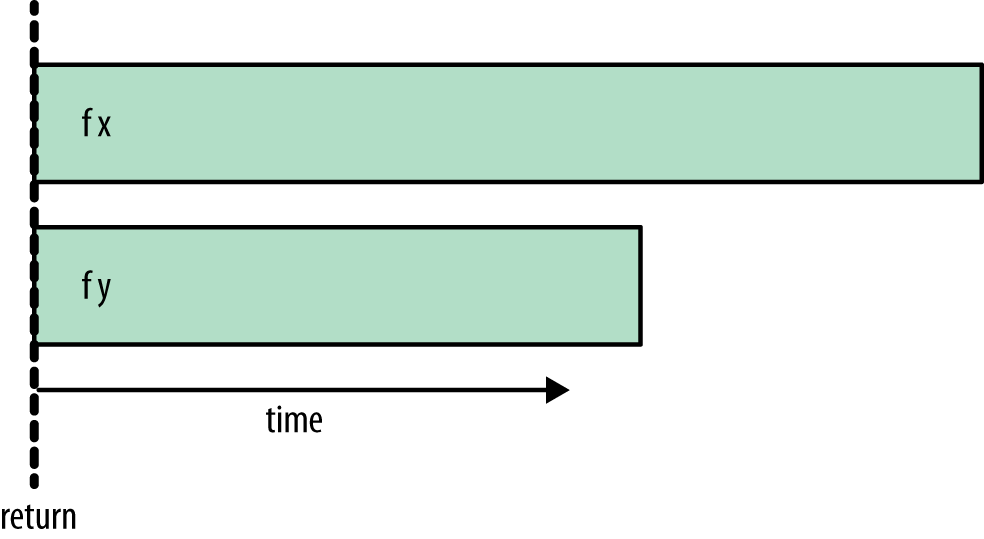
\includegraphics[width=\textwidth]{concurrency_eval1.png}
          \pause
    \item
          Возвращаем пару, когда оба компонента вычислены до WHNF:
          \begin{haskell}
            runEval $ do
              a <- rpar (f x)
              b <- rseq (f y)
              rseq a
              pure (a, b)
          \end{haskell}
          %    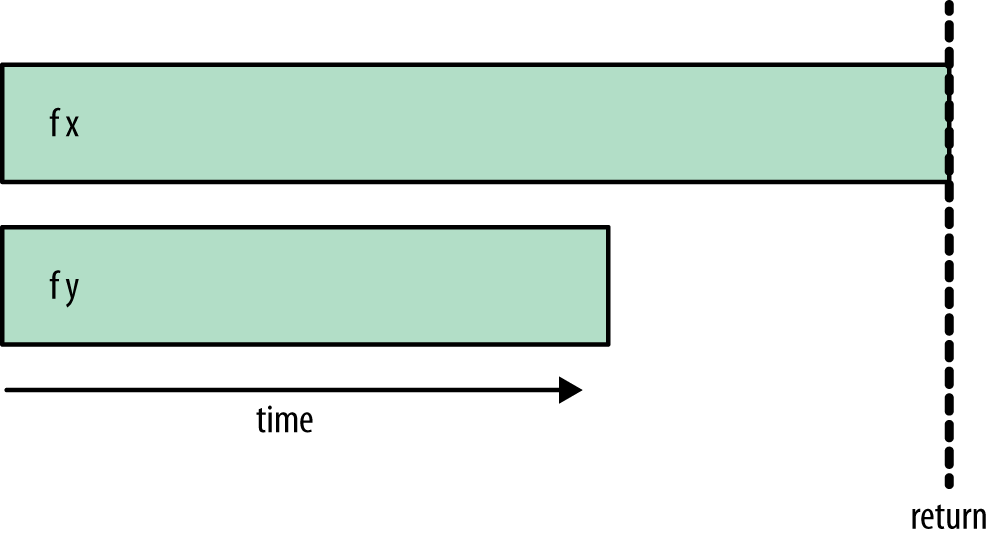
\includegraphics[width=\textwidth]{concurrency_eval2.png}
  \end{itemize}
\end{frame}

\begin{frame}[fragile]
  \frametitle{Фибоначчи в \haskinline|Eval|}
  \begin{itemize}
    \item
          \begin{haskellsmall}
            parFib1 :: Integer -> Integer
            parFib1 0 = 1
            parFib1 1 = 1
            parFib1 n = runEval $ do !\pause!
              f1 <- rpar (parFib1 (n - 1))
              f2 <- rseq (parFib1 (n - 2))
              -- rseq, чтобы занять текущий поток, можно и rpar
              pure (f1 + f2)
          \end{haskellsmall}
          \pause
    \item
          \begin{haskellsmall}
            parFib2 :: Integer -> Eval Integer
            parFib2 0 = pure 1
            parFib2 1 = pure 1
            parFib2 n = do !\pause!
              f1 <- parEval (parFib2 (n - 1))
              f2 <- parFib2 (n - 2)
              rseq (f1 + f2)
          \end{haskellsmall}
          \pause
    \item Здесь для простоты кода много повторных вычислений!
  \end{itemize}
\end{frame}

\begin{frame}[fragile]
  \frametitle{Чтобы это работало}
  \begin{itemize}
    \item По умолчанию GHC собирает программу с однопоточной средой выполнения, и все \haskinline|rpar| (и \haskinline|forkIO| далее) работают на одном ядре.
    \item Нужны опция компиляции \ghcinline|-threaded| и опция среды выполнения \ghcinline|+RTS -N| (все ядра) или \ghcinline|-N4|:
          \begin{ghcismall}
            ghc -O2 -threaded -rtsopts Fib.hs
            ./Fib +RTS -N -s
          \end{ghcismall}
          (в \ghcinline|package.yaml| лабораторных это \ghcinline|-threaded -rtsopts -with-rtsopts=-N|).
  \end{itemize}
\end{frame}

\begin{frame}[fragile]
  \frametitle{Искры и их цена}
  \begin{itemize}
    \item \ghcinline|+RTS -s| печатает статистику искр: \ghcinline|SPARKS: 1000 (900 converted, 0 overflowed, 0 dud, 50 GC'd, 50 fizzled)|. \emph{Converted} "--- взяты в работу, \emph{fizzled} "--- значение уже вычислено к моменту обработки искры, \emph{GC'd} "--- результат никому не понадобился.
          \pause
    \item Число искр у \haskinline|parFib1| растёт экспоненциально. Многие приходятся на мелкие подзадачи, и накладные расходы могут превысить выигрыш.
    \item Ниже некоторого порога вычисляйте последовательно. Сравните время выполнения при \ghcinline|-N1| и \ghcinline|-N2|.
  \end{itemize}
\end{frame}

% TODO восстановить слайд
%\begin{frame}[fragile]
%\frametitle{Примеры \haskinline|Eval|}
%\begin{columns}
%    \begin{column}{0.5\textwidth}
%        Запуск двух вычислений параллельно:
%\begin{haskell}
%runEval $ do
%  a <- rpar (f x)
%  b <- rpar (f y)
%  return (a, b)
%\end{haskell}
%%    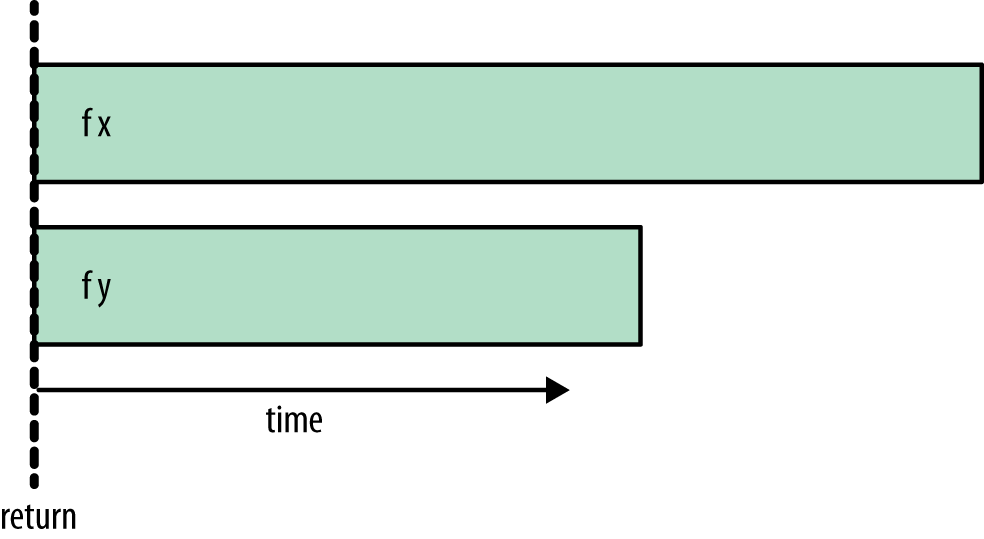
\includegraphics[width=\textwidth]{concurrency_eval1.png}
%    \end{column}\pause
%    \begin{column}{0.5\textwidth}
%    Запуск двух вычислений параллельно и возврат, когда оба закончатся:
%\begin{haskell}
%runEval $ do
%  a <- rpar (f x)
%  b <- rseq (f y)
%  rseq a
%  return (a, b)
%\end{haskell}
%%    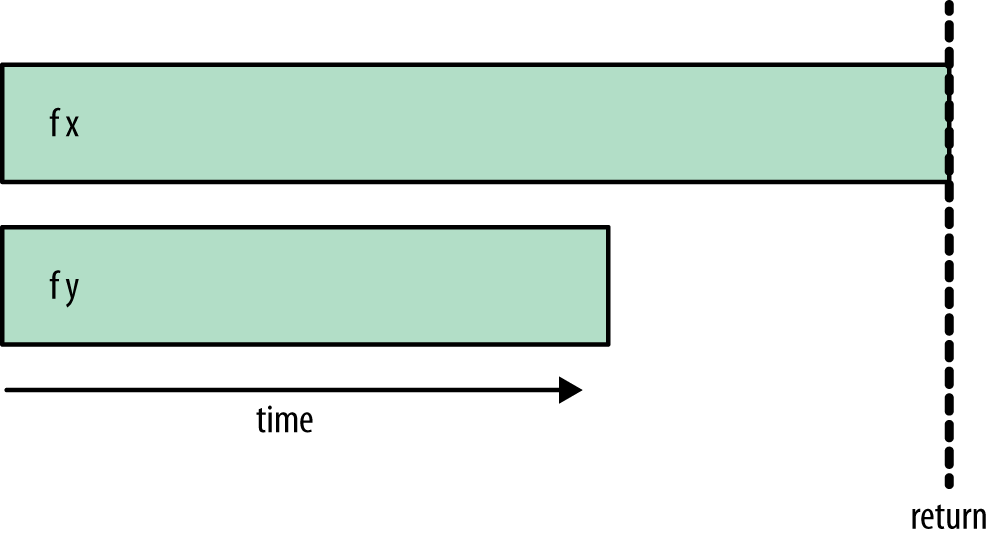
\includegraphics[width=\textwidth]{concurrency_eval2.png}
%    \end{column}
%\end{columns}
%\end{frame}

\begin{frame}[fragile]
  \frametitle{Стратегии вычислений}
  \begin{itemize}
    \item \haskinline|type Strategy a = a -> Eval a|.
    \item \haskinline|rpar| и \haskinline|rseq| --- стратегии.
    \item \haskinline|r0| --- стратегия, которая ничего не вычисляет.
    \item Стратегия принимает на вход thunk, вычисляет его части с помощью \haskinline|r0|, \haskinline|rpar| и \haskinline|rseq|.
    \item Обобщим пример с парой:
          \begin{haskell}
            rparTuple2 :: Strategy (a, b)
            rparTuple2 (a, b) = do !\pause!
              a' <- rpar a
              b' <- rpar b
              return (a', b')
          \end{haskell}
          \pause
          (или \haskinline[fontsize=\small]|rparTuple2 (a, b) = liftA2 (,) (rpar a) (rpar b)|)
    \item
          \begin{haskell}
withStrategy :: Strategy a -> a -> a
withStrategy s x = runEval (s x)
\end{haskell}
  \end{itemize}
\end{frame}

\begin{frame}[fragile]
  \frametitle{Комбинаторы стратегий}
  \begin{itemize}
    \item Обобщим \haskinline|rparTuple2| дальше, чтобы она принимала стратегии на вход:
          \begin{haskell}
            evalTuple2 :: Strategy a -> Strategy b -> 
              Strategy (a, b)
            evalTuple2 strat_a strat_b (a, b) = !\pause! 
              liftA2 (,) (strat_a a) (strat_b b)
          \end{haskell}
          \pause
    \item \haskinline|rparWith :: Strategy a -> Strategy a| запускает стратегию параллельно.
    \item Например, \haskinline|rparWith rseq| эквивалентна \haskinline|rpar|.
          \pause
    \item
          \begin{haskell}
            parTuple2 :: Strategy a -> Strategy b -> 
              Strategy (a, b)
            parTuple2 strat_a strat_b = 
              evalTuple2 (rparWith strat_a) (rparWith strat_b)
          \end{haskell}
  \end{itemize}
\end{frame}

\begin{frame}[fragile]
  \frametitle{Комбинаторы стратегий для списков}
  \begin{itemize}
    \item Применим \haskinline|parList :: Strategy a -> Strategy [a]| к результату \haskinline|map|:
          \begin{haskell}
            parallelMap :: (a -> b) -> [a] -> [b]
            parallelMap f xs = 
              withStrategy (parList rseq) (map f xs)
          \end{haskell}
          \pause
    \item Для списка \haskinline|rseq| вычислит внешний конструктор, \haskinline|rdeepseq| "--- весь список с элементами (нужен \haskinline|NFData|).
    \item Если искр слишком много, пригодятся
          \begin{itemize}
            \item \haskinline|parListChunk|: одна искра на несколько элементов
            \item \haskinline|parBuffer|: добавляет искры по мере потребления списка
          \end{itemize}
  \end{itemize}
\end{frame}

\begin{frame}[fragile]
  \frametitle{Монада \haskinline|Par|: параллелизм без ленивости}
  \begin{itemize}
    \item Модуль \href{https://hackage.haskell.org/package/monad-par/docs/Control-Monad-Par.html}{\haskinline{Control.Monad.Par}} в пакете \haskinline|monad-par|.
    \item Тип \haskinline|Par a| --- тоже монада, описывающая процесс вычисления значения типа \haskinline|a| с параллельными частями.
    \item \haskinline|fork :: Par () -> Par ()| создаёт новый поток.
    \item \haskinline|runPar :: Par a -> a| производит вычисление и возвращает его результат. \pause
    \item Потоки общаются между собой с помощью \haskinline|IVar|, которые можно записать только 1 раз.
    \item В результате не должно быть \haskinline|IVar| или ссылок на них!
    \item При соблюдении этого условия вычисления в \haskinline|Par| детерминированы.
  \end{itemize}
\end{frame}

\begin{frame}[fragile]
  \frametitle{\haskinline|IVar|}
  \begin{itemize}
    \item Интерфейс \haskinline|IVar|:
          \begin{haskell}
            new :: Par (IVar a)
            newFull :: NFData a => a -> Par (IVar a)
            put :: NFData a => IVar a -> a -> Par ()
            get :: IVar a -> Par a
          \end{haskell}
    \item Значения, положенные в \haskinline|IVar|, полностью вычисляются (есть ещё \haskinline|newFull_| и \haskinline|put_|).
    \item Переменной можно дать значение только 1 раз, иначе исключение.
    \item При вызове \haskinline|get| для переменной, ещё не имеющей значения, начинается ожидание.
  \end{itemize}
\end{frame}

\begin{frame}[fragile]
  \frametitle{Примеры \haskinline|Par|}
  \begin{itemize}
    \item \haskinline|spawn :: NFData a => Par a -> Par (IVar a)|: аналог \haskinline|fork|, но возвращающий переменную, в которой будет сохранено вычисленное значение
          \begin{haskell}
            spawn par = do
              var <- new
              fork $ do { x <- par; put var x }
              return var
          \end{haskell}
    \item Параллельный \haskinline|map|:
          \begin{haskell}
            parallelMap :: NFData b => (a -> b) -> [a] -> [b]
            parallelMap f xs = runPar $ do
              ivars <- traverse (\x -> spawn (pure (f x))) xs
              traverse get ivars
          \end{haskell}
          Как и в прошлый раз, создаёт \enquote{поток} для каждого элемента, для простоты кода.
  \end{itemize}
\end{frame}

\begin{frame}[fragile]
  \frametitle{Фибоначчи в \haskinline|Par|}
  \begin{itemize}
    \item[]
    \begin{haskell}
      parFib :: Integer -> Par Integer
      parFib 0 = pure 1
      parFib 1 = pure 1
      parFib n = do !\pause!
        f1var <- spawn (parFib (n - 1))
        f2 <- parFib (n - 2)
        f1 <- get f1var
        pure (f1 + f2)
    \end{haskell}
  \end{itemize}
\end{frame}

\begin{frame}[fragile]
  \frametitle{Конкурентность}
  \begin{itemize}
    \item Перейдём от параллелизма к конкурентности.
    \item Модуль \href{https://hackage.haskell.org/package/base/docs/Control-Concurrent.html}{\haskinline{Control.Concurrent}} в пакете \haskinline|base| и его подмодули \href{https://hackage.haskell.org/package/base/docs/Control-Concurrent-MVar.html}{\haskinline{MVar}}, \href{https://hackage.haskell.org/package/base/docs/Control-Concurrent-Chan.html}{\haskinline{Chan}}, \href{https://hackage.haskell.org/package/base/docs/Control-Concurrent-QSem.html}{\haskinline{QSem}}, \href{https://hackage.haskell.org/package/base/docs/Control-Concurrent-QSemN.html}{\haskinline{QSemN}}.
    \item \haskinline|ThreadId| --- ссылка на поток.
    \item \haskinline|forkIO :: IO () -> IO ThreadId| создаёт новый поток, который произведёт данные действия и выйдет, возвращает ссылку на созданный поток.
          \pause
    \item Это так называемый \enquote{зелёный поток}, то есть не поток операционной системы, а похожий по поведению объект виртуальной машины Haskell.
  \end{itemize}
\end{frame}

\begin{frame}[fragile]
  \frametitle{\haskinline|forkIO|: подводные камни}
  \begin{itemize}
    \item Когда \haskinline|main| завершается, программа завершается целиком: остальные потоки просто убиваются. Дождаться их "--- ваша забота (\haskinline|MVar| на следующем слайде или \hackage{async}).
    \item Необработанное исключение завершает дочерний поток. Вызов \haskinline|forkIO| сам по себе не передаёт это исключение родителю.
    \item Как и для \haskinline|Eval|, второе ядро появится только с \ghcinline|-threaded| и \ghcinline|+RTS -N|; без них зелёные потоки всё равно работают, но по очереди на одном ядре.
  \end{itemize}
\end{frame}

\begin{frame}[fragile]
  \frametitle{\haskinline|MVar|}
  \begin{itemize}
    \item Потоки могут взаимодействать через \haskinline|MVar|, которые очень похожи на \haskinline|IVar|, но записанное значение можно убрать или изменить.
    \item Переменная в любой момент или пустая или полная (содержит значение).
          \begin{haskellsmall}
            newEmptyMVar :: IO (MVar a)
            newMVar :: a -> IO (MVar a)
            putMVar :: MVar a -> a -> IO ()
            readMVar :: MVar a -> IO a
            takeMVar :: MVar a -> IO a
            isEmptyMVar :: MVar a -> IO Bool
          \end{haskellsmall}
    \item \haskinline|putMVar| ждёт, если переменная полна.
    \item \haskinline|takeMVar| и \haskinline|readMVar| отличаются тем, что первая убирает прочитанное значение. На пустой переменной обе ждут.
  \end{itemize}
\end{frame}

\begin{frame}[fragile]
  \frametitle{Фибоначчи с \haskinline|MVar|}
  \begin{itemize}
    \item \haskinline|putMVar| может передать отложенное вычисление. \haskinline|evaluate| из \href{https://hackage.haskell.org/package/base/docs/Control-Exception.html}{\haskinline{Control.Exception}} вычислит сумму в текущем потоке.
          \begin{haskellsmall}
            parFib :: Integer -> IO Integer
            parFib 0 = pure 1
            parFib 1 = pure 1
            parFib n = do !\pause!
              f1var <- newEmptyMVar
              forkIO $ do
                f1' <- parFib (n - 1)
                putMVar f1var f1'
              f2 <- parFib (n - 2)
              f1 <- readMVar f1var
              evaluate (f1 + f2)
          \end{haskellsmall}
    \item Что, если поток упадёт до \haskinline|putMVar|?\pause{} Родитель может остаться ждать в \haskinline|readMVar|.
  \end{itemize}
\end{frame}

\begin{frame}[fragile]
  \frametitle{Фибоначчи: сколько нужно сложений?}
  \begin{itemize}
    \item При вычислении \haskinline|parFib 4| одна ветвь вычисляет \haskinline|parFib 2| напрямую, а другая "--- внутри \haskinline|parFib 3|.
    \item Сколько сложений нужно, если хранить два соседних числа Фибоначчи? \pause
    \item Начнём с пары \haskinline|(1, 1)|, как в наших примерах. Каждый переход от \haskinline|(a, b)| к \haskinline|(b, a + b)| даёт следующее число за одно сложение.
    \item Для $n \ge 1$ достаточно $n-1$ сложений. Распараллеливание исходной рекурсии сохраняет повторные вычисления.
  \end{itemize}
\end{frame}

\begin{frame}[fragile]
  \frametitle{\haskinline|Chan|}
  \begin{itemize}
    \item \haskinline|MVar| можно рассматривать как каналы, хранящие не более одного значения.
    \item \haskinline|Chan| это канал для произвольного количества значений.
          \begin{haskell}
        newChan :: IO (Chan a)
        writeChan :: Chan a -> a -> IO () 
        readChan :: Chan a -> IO a
    \end{haskell}
    \item \haskinline|writeChan| сохраняет значение в конец очереди.
    \item \haskinline|readChan| читает из её начала и ждёт, если она пуста.
  \end{itemize}
\end{frame}

\begin{frame}[fragile]
  \frametitle{Пакет \hackage{async}}
  \begin{itemize}
    \item[]
          \begin{haskellsmall}
            import !\href{https://hackage.haskell.org/package/async/docs/Control-Concurrent-Async.html}{\texttt{Control.Concurrent.Async}}!
            async :: IO a -> IO (Async a)
            wait  :: Async a -> IO a
            withAsync :: IO a -> (Async a -> IO b) -> IO b
            concurrently :: IO a -> IO b -> IO (a, b)
            race :: IO a -> IO b -> IO (Either a b)
            mapConcurrently :: Traversable t =>
              (a -> IO b) -> t a -> IO (t b)
          \end{haskellsmall}
    \item \haskinline|wait| передаёт результат или исключение. \haskinline|withAsync| отменяет поток при выходе из блока.
    \item \haskinline|concurrently| ждёт оба результата, при исключении отменяет второе действие.
    \item \haskinline|race| отменяет проигравшее действие.
  \end{itemize}
\end{frame}

\begin{frame}[fragile]
  \frametitle{Транзакции}
  \begin{itemize}
    \item Как и в базах данных, изменения транзакции вступают в силу все вместе.
    \item В Haskell это позволяет делать монада \href{https://hackage.haskell.org/package/stm/docs/Control-Concurrent-STM.html}{\haskinline{STM}} (пакет \hackage{stm}) с операциями над \haskinline|TVar|:
          \begin{haskellsmall}
            newTVar :: a -> STM (TVar a)
            readTVar :: TVar a -> STM a
            writeTVar :: TVar a -> a -> STM ()
            retry :: STM a
            check :: Bool -> STM ()
            atomically :: STM a -> IO a
          \end{haskellsmall}
    \item \haskinline|check False| вызывает \haskinline|retry|: транзакция может повториться, когда изменится одна из прочитанных ею \haskinline|TVar|.
  \end{itemize}
\end{frame}

\begin{frame}[fragile]
  \frametitle{Перевод между счетами}
  \begin{itemize}
    \item Переведём положительную сумму, когда на счёте отправителя хватит средств.
          \begin{haskellsmall}
            transfer :: TVar Integer -> TVar Integer
                     -> Integer -> STM ()
            transfer from to amount =!\pause! do
              balance <- readTVar from
              check (balance >= amount)
              writeTVar from (balance - amount)
              credit <- readTVar to
              writeTVar to (credit + amount)
          \end{haskellsmall}
          \pause
    \item \haskinline|atomically (transfer from to amount)| проводит обе записи вместе. Другие потоки не увидят перевод, в котором деньги уже списаны, но ещё не зачислены.
  \end{itemize}
\end{frame}

\begin{frame}[fragile]
  \frametitle{Дополнительное чтение}
  \small
  \begin{itemize}
    \setlength{\itemsep}{1pt}
    \item \href{https://simonmar.github.io/pages/pcph.html}{Parallel and Concurrent Programming in Haskell} (бесплатная книга, 2013)
    \item \href{https://www.microsoft.com/en-us/research/wp-content/uploads/2016/02/parallel_haskell2.pdf}{A Tutorial on Parallel and Concurrent Programming in Haskell}
    \item \href{https://learntla.com/intro/conceptual-overview.html}{Learn TLA+}. Поиск гонки между банковскими переводами.
    \item \href{https://erlang.org/}{Erlang}. Язык на основе акторов, которые обмениваются сообщениями.
    \item \href{https://stackoverflow.com/questions/23326920/difference-between-par-monad-and-eval-monad-with-deepseq/23428610#23428610}{Разница между \haskinline|Eval| и \haskinline|Par|} (см. также главу 4 книги Марлоу).
    \item \href{https://hackage.haskell.org/package/streamly}{Streamly}. Конкурентная обработка потоков данных.
    \item \href{https://hackage.haskell.org/package/lvish}{lvish}. Обобщение \haskinline|Par| на основе теории решёток (2014).
  \end{itemize}
\end{frame}

\end{document}
